\documentclass[tikz]{standalone}
\begin{document}
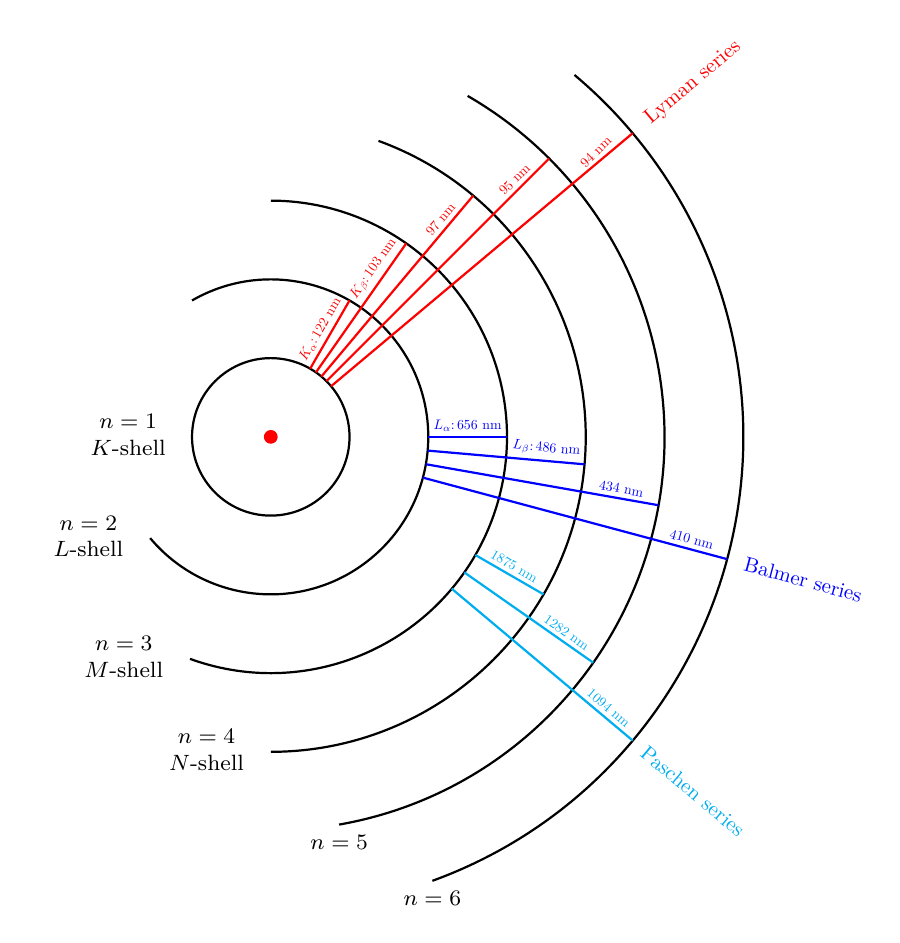
\begin{tikzpicture}

%états d'énergies

\filldraw[red] (0,0)circle(0.08);
\draw[thick] (0,0)circle(1);
\node[left] at (180:1) {
    \footnotesize
    \begin{tabular}{c}
        \(n=1\)\\
        \(K\)-shell
    \end{tabular}
};
\draw[thick] (220:2)node[left] {
    \footnotesize
    \begin{tabular}{c}
        \(n=2\)\\
        \(L\)-shell
    \end{tabular}
}arc(220:480:2);
\draw[thick] (250:3)node[left] {
    \footnotesize
    \begin{tabular}{c}
        \(n=3\)\\
        \(M\)-shell
    \end{tabular}
}arc(250:450:3);
\draw[thick] (270:4)node[left] {
    \footnotesize
    \begin{tabular}{c}
        \(n=4\)\\
        \(N\)-shell
    \end{tabular}
}arc(270:430:4);
\draw[thick] (280:5)node[below] {\footnotesize $n=5$}arc(280:420:5);
\draw[thick] (290:6)node[below] {\footnotesize $n=6$} arc(290:410:6);

%série de Lyman

\draw[red, thick] (60:1)--(60:2) node[midway, above, rotate=60, scale=0.5] {\(K_\alpha\colon 122\) nm};
\draw[red, thick] (55:1)--(55:2) (55:2)--(55:3) node[midway, above, rotate=55,scale=0.5] {\(K_\beta\colon 103\) nm};
\draw[red, thick] (50:1)--(50:3) (50:3)--(50:4) node[midway, above, rotate=50,scale=0.5] {$97$ nm};
\draw[red, thick] (45:1)--(45:4) (45:4)--(45:5) node[midway, above, rotate=45,scale=0.5] {$95$ nm};
\draw[red, thick] (40:1)--(40:5) (40:5)--(40:6) node[midway, above, rotate=45,scale=0.5] {$94$ nm};
\node[rotate=40, red, scale=0.75] at (40:7) {Lyman series};

%série de Balmer

\draw[blue, thick] (0:2)--(0:3) node[above, midway, scale=0.5] {\(L_\alpha\colon 656\) nm};
\draw[blue, thick] (-5:2)--(-5:3) (-5:3)--(-5:4) node[above, midway, scale=0.5, rotate=-5] {\(L_\beta\colon 486\) nm};
\draw[blue, thick] (-10:2)--(-10:4) (-10:4)--(-10:5) node[above, midway, scale=0.5, rotate=-10] {434 nm};
\draw[blue, thick] (-15:2)--(-15:5) (-15:5)--(-15:6) node[above, midway, scale=0.5, rotate=-15] {410 nm};
\node[rotate=-15, blue, scale=0.75] at (-15:7) {Balmer series};

%série de Paschen

\draw[cyan, thick] (-30:3)--(-30:4) node[above, midway, scale=0.5, rotate=-30] {1875 nm};
\draw[cyan, thick] (-35:3)--(-35:4) (-35:4)--(-35:5) node[above, midway, scale=0.5, rotate=-35] {1282 nm};
\draw[cyan, thick] (-40:3)--(-40:5) (-40:5)--(-40:6) node[above, midway, scale=0.5, rotate=-40] {1094 nm};
\node[rotate=-40, cyan, scale=0.75] at (-40:7) {Paschen series};
\end{tikzpicture}
\end{document}